

\begin{flushleft}
The system is to be a modular system which allows for:
\end{flushleft}

\begin{itemize} 
\item[$\bullet$] Only a subset of modules to be deployed. Minimally the system will require the core modules to be deployed.
\item[$\bullet$] Further modules to be added at a later stage.
\end{itemize}

\begin{flushleft}
To this end there should be:
\end{flushleft}

\begin{itemize} 
\item[$\bullet$] Minimal dependencies between modules, and
\item[$\bullet$] No dependencies of core modules on any add-on modules.
\end{itemize}

\begin{flushleft}
Modular design allows that each module encapsulates information that is not available to the rest of the program. This information hiding reduces the cost of subsequent design changes when future functionality is added to STORM. For example, if at a later stage functionality is added to allow for personality tests to be completed within STORM and results are automatically pulled in, a new module can be added without affecting other modules.
\end{flushleft}

\begin{figure}[h]
\centering
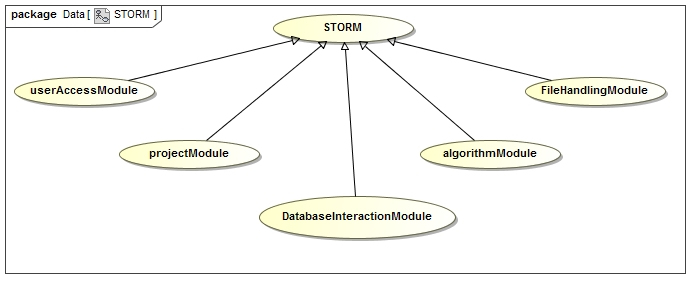
\includegraphics[width=15cm]{./graphics/stormOverview.jpg}
\caption{High level overview of STORM}
\end{figure}